\subsection{Modeling}
\label{sec:Modeling}

\subsubsection{The Classifier}

For training the Gradient Boosting Algorithm, the \emph{GradientBoostingClassifier} class from 
the scikit learn Python library is used. It is part of a group of classes offering different ensemble methods.
As explained in section \ref{sec:Gradient Boosting}, ensemble methods combine the predictions of several
weak learners to generate a more robust model and reduce overfitting issues.
sklearn supports averaging methods like Bagging and Random Forests, which take the average of each learners prediction
as their output. It also supports Boosting Methods like AdaBoost or Gradient Boosting, which
build base estimators sequentially, improving the output each time.
sklearn also provides a classifier and regressor model for each method.

The Gradient Boosting Classifier supports binary and multi-class classification and uses
20 hyperparameters to control the size of each regression tree, the number of trees,
the learning rate and many more.
As explaining and tuning all 20 hyperparameters of the classifier would be beyond the scope of this
paper, three important parameters are explained and optimized.

\begin{itemize}
    \item \textbf{learning\_rate}
    
    As explained in section \ref{sec:Gradient Boosting Algorithm}, the learning rate is used to control how
    much each tree contributes to the result, by multiplying it with the output values of the previous 
    tree. The default value here is $0.1$
    \item \textbf{n\_estimators}

    The number of weak learners (here regression trees) to be used while boosting. The default is $100$.
    \item \textbf{max\_depth}

    The maximum depth of each regression tree. This also impacts its number of nodes.
    The default value is $3$.
\end{itemize}

\subsubsection{Validation Curves}

During hyperparameter tuning, grid search is used to find the optimal value for each parameter.
As this is very resource intensive, a sensible range of values to search in must be found beforehand.
Validation curves can be used to see, how a model's score changes when modulating a single hyperparameter.
Here, an important distinction between the training and cross-validation score has to be made.
The training score is the accuracy the model achieves, when being scored on the same data it was trained on.
A very high training score could be a sign of overfitting.
The cross-validation score (cv score) is the mean accuracy achieved during 5-fold cross validation and is a good measure
of the actual performance of the model.


Figure \ref{fig:Validation Curves modulating 3 hyperparameters} shows the curves for each hyperparameter. The shaded
areas around the graph are the standard deviation, while the graph itself represents the mean score between 5 folds.

Figure \ref{fig:Validation Curves modulating 3 hyperparameters}a shows the best cv score with a learning rate
between 0 and 0.2, declining as it approaches one.
The training score rises as the learning rate increases, which indicates, that the model becomes less generalizable and
more overfitted as the learning rate increases.
Because of these results, only values between 0.01 and 0.25 are considered during hyperparameter tuning.

The cv score stays relatively flat as the number of estimators goes beyond 25 (figure \ref{fig:Validation Curves modulating 3 hyperparameters}).
The training score increases slightly.
This indicates, that a training score close to, but above 25 might be optimal. As the results are not very clear,
a range between 50 and 200 is used for optimization.

For \emph{max\_depth}, the cv score stays relatively flat between 2 and 13 (figure \ref{fig:Validation Curves modulating 3 hyperparameters}).
The training score, on the other hand, increases rapidly from 0 to 7.5, where it reaches its maximum.
Because of this, a range between 2 and 6 is used for hyperparameter tuning.

\begin{figure}[H]
    \centering
    \subfloat[\centering learning\_rate]{{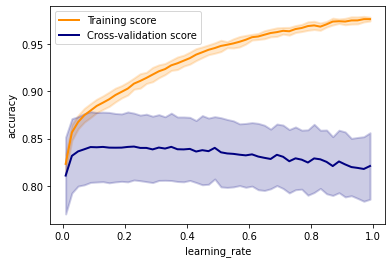
\includegraphics[width=0.45\textwidth]{validation_curve_learning_rate} }}%
    \qquad
    \subfloat[\centering n\_estimators]{{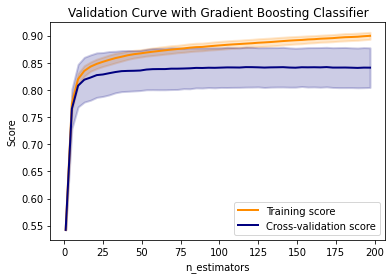
\includegraphics[width=0.45\textwidth]{validation_curve_n_estimators} }}%
    \qquad
    \subfloat[\centering max\_depth]{{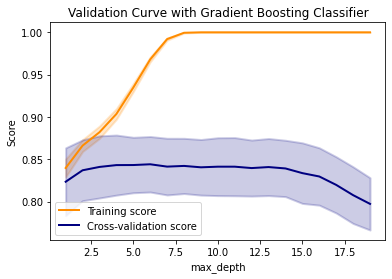
\includegraphics[width=0.45\textwidth]{validation_curve_max_depth} }}%
    \caption{Validation Curves modulatng 3 hyperparameters}%
    \label{fig:Validation Curves modulating 3 hyperparameters}%
\end{figure}

\subsubsection{Hyperparameter Tuning and Fitting a Model}

The parameter grid is given as a Python dictionary containing the parameter name as keys and a list of values for
each key. All undefined hyperparameters are kept at default.
The grid used for training with the value ranges found above looks like this:

\begin{lstlisting}[language=Python]
    param_grid = {
        "learning_rate": [0.01, 0.04, 0.07, 0.1, 0.13, 0.16, 0.19, 0.22, 0.25],
        "n_estimators": [50, 75, 100, 125, 150, 175, 200],
        "max_depth": [2, 3, 4, 5, 6]
    }
\end{lstlisting}

The grid and a \emph{GradientBoostingClassifier} object are passed into a \emph{GridSearchCV} object
which executes the grid search using 5-fold CV.

\begin{lstlisting}[language=Python]
    gbc = GradientBoostingClassifier(random_state=45)    
    search = GridSearchCV(gbc, param_grid,
        n_jobs=-1,
        error_score="raise",
        verbose=1)
\end{lstlisting}

The search object's fit method combines cross-validation, hyperparameter tuning and classifier
fitting to find the best possible combination of hyperparameters to the estimator for the given dataset.
This is done in the following way:

\begin{enumerate}
    \item An estimator is created using the first combination of hyperparameters.
    \item The training set is split into five folds and each fold is used once for calculating accuracy,
    with the other four used for training. The average of the five scores is used as the final score for
    this specific set of parameters.
    \item The score is saved together with the parameters
    \item These steps are repeated with every possible combination of parameters from the 
    parameter grid. This results in a score for every set of parameters.
    \item As every model was fitted using the same method, it is clear that the model with the highest
    score is using the best hyperparameters. A new model is trained without cross-validation using all
    available training data, to create the final model.
\end{enumerate}

The complete standardized dataset is split in 80\% train and 20\% test data.
The samples are shuffled before splitting to ensure an even distribution of data.
Then features and labels are seperated for input into the classifier.

\begin{lstlisting}[language=Python]
    train, test = train_test_split(df_s, test_size=0.2, random_state=45, shuffle=True)

    X_train = train[features]
    X_test = test[features]
    y_train = train["target"]
    y_test = test["target"]
\end{lstlisting}

Then hyperparameter tuning and estimator fitting is started using the training features and labels.

\begin{lstlisting}[language=Python]
    search.fit(X_train, y_train)
\end{lstlisting}

The parameter grid above has 315 possible combinations. As each is fitted on five sets of folds,
there are 1575 models fitted in total during this process.

The resulting model with the best cross-validation score used the following parameters:
\begin{itemize}
    \item learning\_rate: 0.1
    \item n\_estimators: 100
    \item max\_depth: 3
\end{itemize} 

Calculating the accuracy of the resulting model using the test set resulted in an accuracy score of $0.8591$.

A weakpoint of the parameter grid used is, that the values for \emph{n\_estimators} are spread by increments of 25,
leaving possible room for improvement.
To check, if the model could be improved, another parameter grid was used:

\begin{lstlisting}[language=Python]
    param_grid = {
        "learning_rate": [0.01, 0.04, 0.07, 0.1, 0.13, 0.16, 0.19, 0.22, 0.25],
        "n_estimators": [97, 98, 99, 100, 101, 102, 103],
        "max_depth": [2, 3, 4, 5, 6]
    }
\end{lstlisting}

This did not deliver a better result.

Even though a broad spectrum of values was given in the search grid, the optimal values 
are equal to the default parameters for the estimator set by \emph{sklearn}.
This might suggest, that the developers set the default values using a similar dataset to the one used in this project.

Although many combinations were evaluated, there is still a possibility, that this is a local 
maximum and a set of hyperparameters that is far different from the ones tested here are actually
optimal. 